%%Author: Javangers Team

\documentclass[letterpaper,12pt]{report}

%% page layouts
\usepackage[margin=0.8in]{geometry}

%% appendices
\usepackage[toc,page]{appendix}

%enumitem to itemize nicely
\usepackage{enumitem}

%source code highlighting
\usepackage{listings}
\usepackage{lstautogobble}
\usepackage{xcolor}

\usepackage[hidelinks]{hyperref}
\hypersetup{
    linktoc=all,     %sections and subsections linked
    urlcolor=blue
}

% display backtick
\usepackage{upquote}

% import images
\usepackage{graphicx}

\definecolor{lightgray}{rgb}{.95,.95,.95}

% gnu make listing
\lstdefinestyle{bash}{
   language=bash,
   keywordstyle=\bfseries\color{green!40!black},
   commentstyle=\itshape\color{purple!40!black},
   identifierstyle=\color{blue},
   extendedchars=true,
   basicstyle=\ttfamily,
   showstringspaces=false,
   showspaces=false,
   breaklines=true,
   showtabs=false,
   frame=single,
   stringstyle=\color{red},
   backgroundcolor=\color{lightgray},
   autogobble=true,
   aboveskip=-4pt
}

% gnu make listing
\lstdefinestyle{make}{
   language=[gnu]make,
   keywordstyle=\bfseries\color{green!40!black},
   commentstyle=\itshape\color{purple!40!black},
   identifierstyle=\color{blue},
   extendedchars=true,
   basicstyle=\ttfamily,
   showstringspaces=false,
   showspaces=false,
   breaklines=true,
   showtabs=false,
   frame=single,
   stringstyle=\color{red},
   backgroundcolor=\color{lightgray},
   autogobble=true,
   aboveskip=-4pt
}

% ocaml listing
\lstdefinestyle{caml}{
   language=[Objective]Caml,
   keywordstyle=\bfseries\color{green!40!black},
   commentstyle=\itshape\color{purple!40!black},
   identifierstyle=\color{blue},
   extendedchars=true,
   basicstyle=\ttfamily,
   showstringspaces=false,
   showspaces=false,
   breaklines=true,
   showtabs=false,
   frame=single,
   stringstyle=\color{red},
   backgroundcolor=\color{lightgray},
   autogobble=true,
   aboveskip=-4pt
}

% settings for SOL code listings
\lstdefinestyle{sol}{
   language=Java,
   morekeywords={func, construct, shape, string},
   keywordstyle=\bfseries\color{green!40!black},
   commentstyle=\itshape\color{purple!40!black},
   identifierstyle=\color{blue},
   extendedchars=true,
   basicstyle=\ttfamily,
   showstringspaces=false,
   showspaces=false,
   breaklines=true,
   showtabs=false,
   frame=single,
   stringstyle=\color{red},
   backgroundcolor=\color{lightgray},
   autogobble=true,
   aboveskip=-10pt
}

\begin{document}

%% Title, authors and addresses
\title{{\small better call} {\Huge \textbf{SOL}}\\
    \begin{center}{SHAPE ORIENTED LANGUAGE FINAL REPORT}\end{center}
}

\author{
\begin{tabular}{ lc lc lc }
Aditya Narayanamoorthy & \texttt{an2753}  & \textit{Language Guru}    \\
Erik Dyer              & \texttt{ead2174} & \textit{System Architect} \\
Gergana Alteva         & \texttt{gla2112} & \textit{Program Manager}  \\
Kunal Baweja           & \texttt{kb2896}  & \textit{Tester}
\end{tabular}
}

%% Generate the title
\maketitle

%% Table of contents
\tableofcontents{}

\chapter{Introduction}
  SOL (Shape Oriented Language), is a domain specific programming language that allows programmers to create 2D animations with ease, through an object-oriented approach. Engineers, programmers, scientists and designers, through SOL, have the ability to define and create objects, known as Shapes, and dictate their appearance and movements on the screen. In addition, SOL\'s simplicity saves developers the trouble of learning complicated third-party animation tools, without sacrificing control over behavior of objects. It compiles into LLVM IR bytecode, making it adaptable across different architectures. The produced LLVM IR bytecode can be translated further into assembly code and linked statically against a predefined library before compiling down into an executable for a specific architecture using the LLVM compiler and GCC compilers respectively. The predefined library used by SOL for graphic rendering has been built on top of SDL2, that abstracts away the lower level details for drawing and animating objects.

  \section{Background}
  SOL takes its inspiration from the ease of programming in \textit{object-oriented paradigm} and the complexity of existing libraries/solutions for rendering graphics. It attempts to combine both of them and provide a language which allows developers to organize graphics into a collection of \textit{Shapes} (much like objects) which can be easily defined, created and interacted with to produce powerful images and/or animations at a fast paced development.\\

  SOL is commonly used to model various types of scientific data, but it can also be applicable in other domains, such as:
  \begin{enumerate}
    \itemsep 0em
    \item Drawing engineering models
    \item Data visualization
    \item Bored college students making funny memes
    \item Entertaining animations
  \end{enumerate}

\chapter{Language Tutorial}
  This chapter provides a brief description of basic components of the language to guide programmers towards creating their first SOL! It has been divided into three parts:
  \begin{enumerate}
    \item \textbf{Environment setup} - guide to setting up the SOL compiler and development environment
    \item \textbf{Language Quick Tour} - a bried descriptioin of basic components of language.
    \item \textbf{Sample Program} - Create dancing line bars
  \end{enumerate}

  \section{Environment setup}
  SOL compiler has been developed and tested on Ubuntu 15.04 and Ubuntu 16.04 environments, and is capable of supporting others as well. It can work on multiple architectures as the LLVM IR bytecode can further be compiled into architecture specific executables. The environment setup tutorial assumes you have the latest version of SOL compile source code downloaded from our repository.

    \subsection{Building SOL compiler (Ubuntu 15.04 or later version)}
    \begin{enumerate}
      \item SOL compiler is written in OCaml. Download the source code from our github repository: \colorbox{lightgray}{{\href{https://github.com/bawejakunal/sol}{https://github.com/bawejakunal/sol}}}

      \item Download and run the bash script below, which installs the latest compatible version of OCaml compiler and opam for *-nix OS environments.\\
      \colorbox{lightgray}{{\href{https://raw.githubusercontent.com/ocaml/ocaml-ci-scripts/master/.travis-ocaml.sh}{https://raw.githubusercontent.com/ocaml/ocaml-ci-scripts/master/.travis-ocaml.sh}}}

      \item Configure the opam environment for importing Ocaml packages\\
      \colorbox{lightgray}{\lstinline[style=bash]{eval `opam config env`}}

      \item Install LLVM compiler toolchain and ocaml bindings, for the SOL compiler\\
      \colorbox{lightgray}{\lstinline[style=bash]{./install-llvm.sh}}

      \item Download and Install SDL2 and SDL2\_gfx libraries which are used by our predefined static library for graphics rendering.\\
        \colorbox{lightgray}{\lstinline[style=bash]{wget} \href{http://www.ferzkopp.net/Software/SDL2\_gfx/SDL2\_gfx-1.0.3.tar.gz}{http://www.ferzkopp.net/Software/SDL2\_gfx/SDL2\_gfx-1.0.3.tar.gz}}\\
        \colorbox{lightgray}{\lstinline[style=bash]{./install-sdl-gfx.sh}}

      \item Build the SOL compiler as \texttt{sol.native} and the static graphic libarary as \texttt{predefined.o}\\
      \colorbox{lightgray}{\lstinline[style=bash]{make all}}

    \end{enumerate}

  \section{SOL Quick Tour}
  This section provides a quick tour on the data types, data structures and the shape oriented programming paradigm provided by SOL, with examples. Towards the end we walk through the steps to generate an executable SOL program. For a detailed explanation of language syntax, semantics and built-in functions refer to chapter \ref{lrm}.

    \subsection{Primitive data types}
      All variables of primitive data types are declared starting with their type followed by an identification. SOL supports the following primitives:
      \begin{enumerate}
        \itemsep 0em
        \item \texttt{int} - integers
        \item \texttt{float} - double precision floating point number
        \item \texttt{char} - single character from \texttt{ASCII} character set
        \item \texttt{string} - a sequence of one or more \texttt{ASCII} characters
      \end{enumerate}
      Example:\\
      \begin{lstlisting}[style=sol]
        func main() {
            int x;  /* declare primitives */
            float y;
            char c;
            string s;

            x = 5;  /* assign values to primitives */
            y = 6.5;
            c = 'a';
            s = "better call SOL";
        }
      \end{lstlisting}

    \subsection{Arrays and Shapes}
      SOL supports two complex data structures:
      \subsubsection{Array}
        An array is a fixed size sequence of primitives or objects of a given \textit{shape}. Individual elements can be accessed within array by specifying indices as integers in range \texttt{0} to \texttt{1 less than array length}.\\
        Example:\\
        \begin{lstlisting}[style=sol]
          func main() {
              int [3]a;      /* declare array of 3 integers */
              a = [1, 2, 3]; /* init array with 3 elements*/
              a[1] = 4;      /* update second element value to 4 */
              a[2] = a[0];   /* last element equal to first element */
          }
        \end{lstlisting}

      \subsubsection{Shape}
        A collection of one or more variables/arrays of \textit{primitives and/or shapes} which come together to describe a \textit{shape}. These variables are called \textit{member variables} of a shape. A shape definition can also contain function definitions, referred as \textit{member functions}.\\
        Example:\\
        \begin{lstlisting}[style=sol]
          class Line {
              string name;  /* identify a line by name */
              int [2]start; /* first end point of a line */
              int [2]end;   /* other end point of a line */

              /* compulsory constructor for a shape */
              construct(int [2]s, int[2]e) {
                  /* constructor can be empty definition */
                  start = s;
                  end = e;
              }

              /* compulsory draw member function.*/
              draw() {
                  /* accepts no arguments */
                  /* can be empty definition */
              }
          }

          func main() {
              Line l; /* declare a variable of shape Line */
              l = shape Line([1,1], [2,2]); /* instantiate a Line object */
          }
        \end{lstlisting}

    \subsection{Operators}
    SOL supports \texit{arithmetic operations, relational comparisons and logical operations}. For all binary operators described in this section, the operands are specified to the left and right, respectively, of the operator and \textit{both operands must be expressions of same data types}.\\
    All logical operators accept \textit{boolean logic expressions},represented as \textit{integer expression} in SOL. Non-zero expressions correspond to \texttt{true} and a \texttt{zero} corresponds to \texttt{false}. 

    \begin{enumerate}
      \itemsep 0em
      \item \textit{Binary arithmetic operators}: \texttt{+, -, *, / \%}
      \item \textit{Relational operators (binary)}: \texttt{==, |=, >, >=, <, <=}
      \item \textit{Logical operators}: \texttt{\&\&, ||} \textit{(operands must be of type int)}
      \item \textit{Logical not}: \texttt{!} \textit{(unary and right associative)}
      \item \textit{Unary negation}: \texttt{-} \textit{(unary and right associative)}
    \end{enumerate}

    All expressions are evaluated left to right. Please refer to section \ref{precedence} for exact order of preference and associativity rules for each operator.\\

    Example:\\
    \begin{lstlisting}[style=sol]
        func main() {
            int x;
            int y;
            int c;
            float f;
            float g;

            x = 2;
            y = 3;
            f = 3.0;
            g = 6.0;

            y = x + y;  /*5: integer addition */
            x = y - x;  /*3: subtraction */

            g = g * f;  /* 18: floating point multiplication*/
            f = g / f;  /* 6: floating point division */
            y = y % 2;  /*1: modulo operation */

            c = g == f; /*0: EQUALITY is false */
            c = g != f; /*1: NOT EQUAL is true */
            c = g > f;  /*1: g GREATER THAN f */
            c = y >= x; /*1: y GREATER THAN OR EQUAL x is true */
            c = y < x;  /*0: y LESS THAN x is false */
            c = 5 <= 5; /*1: 5 LESS THAN OR EQUALS 5 is true */

            c = 5 && 0; /*0: LOGICAL AND of true and false */
            c = 2 || 0; /*1: LOGICAL OR of true and false */

            c = !c;   /*0: LOGICAL NOT of true(1) */
            f = -f;   /*-6: unary negation of arithmetic expression */
        }
    \end{lstlisting} 

    \subsection{Control flow statements}
    SOL program statements are executed in order, with the entry point being the main function. However, sometimes developers need to execute only a branch of source code (jump through some statements) or execute a portion of code repeatedly. SOL provides two control flow statements if and while for conditional branching and looping through a portion of code, respectively.

      \subsubsection{if-statement}
      An \textit {if statement block} allows to execute or skip a \texit{code branch} based on a \textit{logical expression}.\\
      Example:\\
      \begin{lstlisting}[style=sol]
        func main() {
          if (1 > 2) {
            /* condition if false; skip this code block */
            consolePrint("NOT PRINTED");
          }
          consolePrint("Hello World");
        }
      \end{lstlisting}

      \subsubsection{while-statement}
      A \texit{while statement block} allows to execute a portion of source code repeatedly until a logical condition, in predicate, is no longer satisfied.
      \begin{lstlisting}[style=sol]
        func main() {
            int i;
            i = 1;
            while (i <= 5) {
                consolePrint("Hello");  /* this loop prints Hello 5 times*/
                i = i + 1;    /* loop terminates when i exceeds 5 */
            }
        }
      \end{lstlisting}

    \subsection{Functions in SOL}
    In SOL functions can be defined as a way to abstract away and re-use a code lock, with a named representation. These are useful if a particular piece of code needs to be executed at multiple places in the program. Functions in SOL can be defined as stand alone functions or as \textit{member functions} of a \textit{shape} definition. Function definitions begin with the \texttt{func} keyword and they optionally accept arguments as input values and return a result, for which the result type needs to be indicated in the function definition. A function may return no value \textit{(void type)} in which case no return type needs to be mentioned during function definition. Please refer section \ref{function} for a detailed explanation of function definition syntax.\\
    
    Example:\\
    \begin{lstlisting}[style=sol]
      /* define a function that accepts two integers and returns their sum */
      func int add(int x, int y) {
          /* sum of two integers */
          return x + y;
      }

      func main() {
          int sum;
          sum = add(2, 3);
          if (sum == 5) {
              consolePrint("CORRECT");
          }
      }
    \end{lstlisting}

    Functions in SOL also support recursion. SOL also provides a number a of type conversion functions and built-in functions for displaying and animating shapes on screen and printing text on screen or console. Please refer to section \ref{internal} for detailed information, syntax on these functions.

  \section{Dancing Bars Tutorial (Sample SOL program)}
  The following program shows a simple definition of a \textit{dancing line} as a \textit{shape} and uses this definition to create a set of colored bars, that oscillate on one endpoint, at a given frequency.
  \begin{enumerate}
    \itemsep 0em
    \item As SOL treats all animation as an interaction of \textit{shapes}, we first define a thick line \textit{shape} in SOL, which can oscillate in length on one end.\\
    The constructor accepts four main arguments: \texttt{start point}, \texttt{end point}, \texttt{color} and \texttt{frequency} of oscillation\\
    We define its \texttt{draw} function based on these input arguments.\\

    \begin{lstlisting}[style=sol, aboveskip=1pt]
      shape DanceLine {
          int [2]start;
          int [2]end;
          int [3]color;
          int freq;   /* oscillation frequency */
          int cnt;
          int d;      /* length change per iteration */

          /* constructor */
          construct(int [2]s, int [2]e, int[3]clr, int f) {
              start = s;
              end = e;
              color = clr; 
              freq = f;   
              cnt = 0;    /* initial counter */
              d = 2;  
          }

          /* drawing specification for single frame */
          draw(){
              int i;
              int [2]s;   /* control points for drawCurve */
              int [2]m;
              int [2]e;

              /* increment count on each frame */
              cnt = cnt + 1;

              if (cnt > freq) {
                  d = -d;     /* reverse direction */
                  cnt = 0;    /* reset freq counter */
              }

              /* change object length on one end */
              end[1] = end[1] + d;

              s = start;  /* end points of line */
              e = end;

              /* draw 10 bezier curves for thickness */
              i = 0;
              while (i < 10) {
                  s[0] = s[0] + 1;
                  e[0] = e[0] + 1;

                  /* bezier curve mid point */            
                  m[0] = (s[0] + e[0]) / 2;
                  m[1] = (s[1] + e[1]) / 2;

                  /* draw straight bezier curve */
                  drawCurve(s, m, e, 2, color);
                  i = i + 1;
              }
          }
      }
    \end{lstlisting}

    \item The next step is to create a collection of multiple \textit{DanceLine} instances, say \textit{DiscoBar}. Hence, we define a new \texttt{shape}, \textit{DiscoBars} that defines three variables of \texttt{shape} \textit{DanceLine}. In the constructor, we instantiate the \textit{member variables} with different colored lines oscillating at different frequencies.\\

    \begin{lstlisting}[style=sol, aboveskip=1pt]
      shape DiscoBars {
          DanceLine d1;   /* member variables */
          DanceLine d2;
          DanceLine d3;

          construct () {
              /* instantiate DanceLine member variables */
              d1 = shape DanceLine([100,300], [100,252], [30,144,255], 20);
              d2 = shape DanceLine([130,300], [130,202], [210,105,30], 40);
              d3 = shape DanceLine([160,300], [160,132], [50,205,50], 80);
          }

          draw(){
              /* empty draw function 
               * draw functions of member variables
               * are called implicitly
               */
          }
      }
    \end{lstlisting}
  
    \item As a final step, we need to create one object of \textit{DanceBards} shape in the \textit{main} function, which is the entry point to a SOL program. The SOL runtime will recursively call its \textit{draw} function and \texttt{draw} functions of its member variables at each frame, to display the osciallating lines.\\

    \begin{lstlisting}[style=sol, aboveskip=1pt]
      func main() {
          DiscoBars bars;
          bars = shape DiscoBars();
      }
    \end{lstlisting}
  \end{enumerate}

  Your final output on screen should look like the image shown below, with the colored bars \textbf{oscillating in length, at their upper ends}, at different frequencies.\\
  \begin{center}
      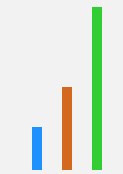
\includegraphics[scale=1]{dancing-bars.png}\\
      \caption{Fig 2.1 DiscoBars Tutorial}
  \end{center}


\chapter{Language Reference Manual} \label{lrm}

  %% include the common content for lrm
  
\section{Introduction}
%% Text of abstract
SOL is a simple language that allows programmers to create 2D animations with ease. Programmers will have the ability to define and create objects, known as shapes, and dictate where they appear, and how they move. SOL uses \textit{point} (visual dot) and \texit{B\'ezier Curves} with three control points as the basic drawing controls provided to the programmer for defining shapes. As a lightweight object-oriented language, SOL allows for unlimited design opportunities and eases the burden of animation. In addition, SOL’s simplicity saves programmers the trouble of learning complicated third-party animation tools, without sacrificing control over behavior of objects.
\par

\section{Conventions}
    The following conventions are followed throughout this SOL Reference Manual.

    \begin{enumerate}
        \itemsep0em
        \item \texttt{literal} - Fixed space font for literals such as commands, functions,\\
        \hspace*{4.4em} keywords, and programming language structures.
        
        \item \textit{variable} - Italics for variables, words, and concepts being defined.
    \end{enumerate}

    The following conventions are applied while drawing and animating objects, using internal functions (see Section \ref{internal}):

    \begin{enumerate}
        \itemsep0em
        \item The origin of the drawing canvas is on the top left of the screen.
        \item The positive X-axis goes from left to right.
        \item The positive Y-axis goes from top to bottom.
        \item Positive angles specify rotation in a clockwise direction.
        \item Coordinates are specified as integer arrays of size 2, consisting of an X-coordinate followed by a Y-coordinate.
        \item Colors are specified as integer arrays of size 3, consisting of Red, Green and Blue values in the range 0 - 255, where \texttt{[0, 0, 0]} is black and \texttt{[255, 255, 255]} is white.
    \end{enumerate}

\section{Lexical Conventions}

This section describes the complete lexical conventions followed for a syntactically correct SOL program, forming various parts of the language.

    \subsection{\textit{Comments}}
    Comments in SOL start with character sequence \texttt{/*} and end at character sequence \texttt{*/}. They may extend over multiple lines and all characters following \texttt{/*} are ignored until an ending \texttt{*/} is encountered.

    \subsection{\textit{Identifiers}}\label{identifer}
    In SOL, an identifier is a sequence of characters from the set of english alphabets, arabic numerals and underscore (\_). The first character of an identifier should always be a lower case english alphabet. Identifiers are case sensitive. Identifiers cannot be any of the reserved keywords mentioned in section \ref{keywords}.

    \subsection{\textit{Keywords}} \label{keywords}
    Keywords in SOL include data types, built-in functions, and control statements, and may not be used as identifiers as they are reserved.

        \begin{center}
            \begin{tabular}{ |c|c|c|c| } 
            \hline
                int     & if            & main          & shape   \\ 
                float   & while         & setFramerate  & \\ 
                char    & func          & getFramerate  & \\
                string  & construct     & print         & \\
                        & return        & consolePrint  & \\
                        &               & intToString   & \\
                        &               & floatToString & \\
                        &               & charToString  & \\
                        &               & render        & \\
                        &               & wait          & \\
                        &               & drawPoint     & \\
                        &               & drawCurve     & \\
                        &               & translate     & \\
                        &               & rotate        & \\

            \hline
            \end{tabular}
        \end{center}

    \subsection{\textit{Integer Constants}}
    A sequence of one or more digits representing a number in base-10, optionally preceded by a unary negation operator (\texttt{-}), to represent negative integers.\\
    Example: \texttt{1234}

    \subsection{\textit{Float Constants}}
    Similar to an integer, a float has an \textit{integer}, a decimal point (\texttt{.}), and a fractional part. Both the integer and fractional part are a sequence of one or more digits. A negative float is represented by a preceding unary negation operator (\texttt{-}).\\
    Example: \texttt{0.55  10.2}

    \subsection{\textit{Character Constants}}
    An ASCII character within single quotation marks.\\
    Example: \texttt{'x' 'a'}

    \subsection{\textit{Escape Sequences}}
    The following are special characters represented by escape sequences.
        \begin{center}
            \begin{tabular}{ |c|c| }
            \hline
                \textbf{Name}   & \textbf{Escape}\\
                \hline
                newline         & \textbackslash n\\
                tab             & \textbackslash t\\
                backslash       & \textbackslash \textbackslash\\
                single quote    & \textbackslash '\\
                double quote    & \textbackslash "\\
                ASCII NUL character & \textbackslash 0\\
            \hline
            \end{tabular}
        \end{center}

    \subsection{\textit{String constants}}
    A SOL \textit{string} is a sequence of zero or more \textit{characters} within double quotation marks.\\
    Example: \texttt{"cat"}

    \subsection{\textit{Operators}}
    SOL has mainly four categories of operators defined below:

        \subsubsection{\textit{Assignment Operator}}
        The right associative \textit{assignment operator} is denoted by the (\texttt{=}) symbol having a variable identifier to its left and a valid expression on its right. The \textit{assignment operator} assigns the evaluated value of expression on the right to the variable on the left.

        \subsubsection{\textit{Unary Negation Operator}} \label{negation}
        The right associative unary negation operator (\texttt{-}) can be used to negate the value of an arithmetic expression.

        \subsubsection{\textit{Arithmetic Operators}}
        The following table describes \texttt{binary arithmetic operators} supported in SOL which operate on two \texttt{arithmetic expressions} specified before and after the operator respectively. The said expressions must both be of type \texttt{int} or \texttt{float}. Please refer to section \ref{precedence} for precedence and associativity rules.

        \begin{center}
            \begin{tabular}{ |c|c| }
            \hline
                \textbf{Operator} & \textbf{Definition} \\
                \hline
                +   &   Addition\\
                -   &   Subtraction\\
                $*$   &   Multiplication\\
                /   &   Division\\
                \%  &   Modulo\\
            \hline
            \end{tabular}
        \end{center}

        \subsubsection{\textit{Comparison Operators}}
        The comparison operators are left associative binary operators for comparing values of operands defined as expressions. Please refer to section \ref{precedence} for precedence and associativity rules.
        \begin{center}
            \begin{tabular}{ |c|c| }
            \hline
                \textbf{Operator} & \textbf{Definition} \\
                \hline
                ==              & Equality \\
                !=              & Not Equals \\
                \textless       & Less than \\
                \textgreater    & Greater than \\
                \textless=      & Less than or equals \\
                \textgreater=   & Greater than or equals \\
            \hline
            \end{tabular}
        \end{center}
        
        \subsubsection{\textit{Logical Operators}}
        The logical operators evaluate boolean expressions and return an integer as result: with 0 as \textit{False} and 1 as \textit{True}. Please refer to section \ref{precedence} for precedence and associativity rules.
        \begin{center}
            \begin{tabular}{ |c|c| }
                \hline
                \textbf{Operator} & \textbf{Definition}\\
                \hline
                \&\&  & AND\\
                $||$  & OR\\
                !  & NOT\\
                \hline
            \end{tabular}
        \end{center}

    \subsection{\textit{Punctuators}}
    The following symbols are used for semantic organization in SOL:
     \begin{center}
        \begin{tabular}{ |p{0.25\hsize}|p{0.75\hsize}| }
            \hline
            \textbf{Punctuator} & \textbf{Usage} \\
            \hline
            \{\}            & Used to denote a block of code. Must be present as a pair. \\
            ()              & Specifies conditions for statements before the subsequent code, or denotes the arguments of a function. Must be present as a pair. \\
            \lbrack\rbrack  & Indicates an array. Must be present as a pair. \\
            ;               & Signals the end of a line of code. \\
            ,               & Used to separate arguments for a function, or elements in an array definition. \\
            \hline
        \end{tabular}
     \end{center}
    
\section{Identifier Scope}
    \subsection{\textit{Block Scope}}
    Identifier scope is a specific area of code wherein an identifier exists. A scope of an identifier is from its declaration until the end of the code block within which it is declared.
    
    \subsection{\textit{File Scope}}
    Any identifier (such as a variable or a function) that is defined outside a code block has file scope i.e. it exists throughout the file.\\
    If an identifier with file scope has the same name as an identifier with block scope, the block-scope identifier gets precedence.

\section{Expressions and Operators}
    \subsection{\textit{Precedence and Associativity}} \label{precedence}
    SOL expressions are evaluated with the following rules:
    \begin{enumerate}
        \itemsep0em
        \item Expressions are evaluated from left to right as operators are left associative, unless stated otherwise.

        \item Expressions within parenthesis take highest precedence and are evaluated prior to substituting in outer expression.
        
        \item The unary negation operator (\texttt{-}) and logical not operator (\texttt{!}) are placed at the second level of precedence, above the binary, comparison and logical operators. It groups right to left as described in section \ref{negation}.
        
        \item The third level of precedence is taken by multiplication (\texttt{*}), division (\texttt{/}) and modulo (\texttt{\%}) operations.
        
        \item Addition (\texttt{+}) and subtraction (\texttt{-}) operations are at the fourth level of precedence.
        
        \item At the fifth level of precedence are the comparison operators: \texttt{\textless, \textgreater, \textless=, \textgreater=}.

        \item At sixth level of precedence are the equality comparison operators: \texttt{==} and \texttt{!=}.

        \item The logical operators, OR (\texttt{||}) and AND (\texttt{\&\&}) take up the next level of precedence.

        \item At the final level of precedence, the right associative assignment operator (\texttt{=}) is placed, which ensures that the expression to its right is evaluated before assigning to the left variable identifier.

    \end{enumerate}
    
    \subsection{\textit{Dot Accessor}}
    To access members of a declared \texttt{shape} (further described in section \ref{classes}), use the dot accessor `.' followed by the identifier name of the \textit{member variable} or \textit{member function}. \\
    Example: \texttt{shape\_object.point1 /* This accesses the variable point1 within the object shape\_object */}


\section{Declaring Identifers}

    Declarations determine how an identifier should be interpreted by the compiler. A declaration should include the identifier type and the given name.

    \subsection{\textit{Type Specifiers}} \label{type}
    SOL provides four type specifiers for data types:
    \begin{itemize}
        \itemsep0em
        \item \textit{int} - integer number
        \item \textit{float} - floating point number
        \item \textit{char} - a single character
        \item \textit{string} - string (ordered sequence of characters)
    \end{itemize}

    \subsection{\textit{Declaring Variables}}
    An identifier, also referred to as a \textit{variable}, is declared by specifying the \texttt{primitive type} or name of the \texttt{Shape}, followed by a valid identifier, as specified in section \ref{identifer}. Variables can be declared only at the beginning of a function or at the top of the source files, as global variables, which are accessible within all subsequent function or shape definitions.

    \subsection{\textit{Array Declarators}} \label{array}
    An array may be formed from any of the primitive types and \texttt{shape}s, but each array may only contain one type of primitive or \texttt{shape}. At declaration, the type specifier and the size of the array must be indicated. The array size need not be specified for strings, which are character arrays. SOL supports \texttt{fixed size arrays}, declared at compile time i.e. a program can not allocate dynamically sized arrays at runtime. Arrays are commonly used in SOL to specify coordinates with two integers and specify drawing colors in RGB format with an array of three integers.\\
    Example: \texttt{int[2] coor; /* Array of two integers */}

    \subsection{\textit{Function Declarators and Definition}} \label{function}
    Functions are declared with the keyword: \texttt{func}. This is followed by the \textit{return type} of the function. If no return type is specified, then the function automatically does not return any value. Functions are given a name (a valid \textit{identifier}) followed by function formal arguments. These arguments are a comma-separated list of variable declarations within parentheses. Primitives are passed into functions by value, and objects and arrays are passed by reference. This function declaration is then followed by the function definition, within curly braces; functions must always be defined immediately after they are declared.\\
    Functions can also be defined within \textit{shape} definitions in which case they are referred as \textit{member functions} of the \textit{shape}. (see section \ref{classes})\\

    Example:\\
    \begin{lstlisting}[style=sol]
        func example(int a, int b){
            /* a function named example that takes
               two arguments, both of type int */
        }
    \end{lstlisting}

    \subsection{\textit{Constructor Declarators}}
    Constructors are declared with the keyword: \texttt{construct}. Constructor definitions are similar to function definitions with three additional constraints: 
    \begin{enumerate}
        \itemsep0em
        \item Constructors are defined inside the \textit{shape} definition
        \item A constructor is defined with the \texttt{construct} keyword, followed by optional formal arguments, within parenthesis as a comma-separated list of variable declarations, similar to function definitions
        \item Constructors do not have a return type specified
    \end{enumerate}
    Example:\\
    \begin{lstlisting}[style=sol]
    shape Point {
        int [2]coordinate;
        construct (int x, int y) {
            /* constructor definition */
            coordinate[0] = x;
            coordinate[1] = y;
        }
    }
    \end{lstlisting}
    Please see section \ref{classes} for defining shapes in SOL and creating shape instances.

    \subsection{\textit{Definitions}}
    A definition of a primitive type variable includes a value, assigned by the assignment operator `\texttt{=}'. For defining arrays, \texttt{rvalue} is the sequence of array literals within square brackets. \textit{Shapes} are objects which are initialized by calling the \texttt{construct}, with optional parameters (see section \ref{classes}). In SOL programs, all variables \textit{must} be \textit{declared} before assigning values.\\
    Example:\\
    \begin{lstlisting}[style=sol]
        char y;       /* declarations */
        float z;
        int [3]w;     /* array declaration */
        string s;
        Triangle t;

        y = 'b';      /* definitions */
        z = 3.4;
        w = [5, 2, 0];
        s = "cats";
        t = shape Triangle();   /* a triangle object */
    \end{lstlisting}

\section{Statements}
A statement in SOL refers to a complete instruction for a SOL program. All statements are executed in order of sequence. The four types of statements are described in detail below:\\

    \subsection{\textit{Expression Statement}}
    Expression statements are those statements that get evaluated and produce a result. This can be as simple as an assignment or a function call.\\
    Example: \texttt{x = 5; /* assign 5 to identifier x */}

    \subsection{\textit{If Statement}}
    An \textit{if} statement is a conditional statement, that is specified with the \texttt{if} keyword followed by an \textit{expression} specified within a pair of parenthesis; further followed by a block of code within curly braces. The code specified within the \texttt{if} block executes if the expression evaluates to a non-zero \textit{integer}.\\
    Example:\\
    \begin{lstlisting}[style=sol]
        int x;
        x = 1;
        if (x == 1) {
            /* This code gets executed */
        }
    \end{lstlisting}

    \subsection{\textit{While Statement}}
    A \textit{while} statement specifies the looping construct in SOL. It starts with the \texttt{while} keyword, followed by an expression specified within a pair of parenthesis; this is followed by a block of code within curly braces which is executed repeatedly as long as the condition in parentheses is valid. This condition is re-evaluated before each iteration and the code within \texttt{while} block executes if the condition evaluates to a non-zero \textit{integer}. \\
    Example:\\
    \begin{lstlisting}[style=sol]
            int x;
            x = 5;
            while (x > 0) {
                /* This code gets executed 5 times */
                x = x - 1;
            }
        \end{lstlisting}

    \subsection{\textit{Return statement}}
    The return statement stops execution of a function and returns to where the function was called originally in the code. Potentially returns a value; this value must conform with the return type specified in the function declaration. If no return type was specified, a \textit{return} statement without any value specified is syntactically valid (but not compulsory).\\
    Example:\\
    \begin{lstlisting}[style=sol]
        func int sum(int x, int y) {
            /* return sum of two integers */
            return x + y;
        }
    \end{lstlisting}
    
\section{Internal Functions} \label{internal}
SOL specifies a set of required/internal functions that must be defined for specific tasks such as drawing, rendering or as an entry point to the program, described below.

    \subsection{\textit{main}}
    Every SOL program must contain a \texttt{main} function as this is the entrypoint of the program. The \texttt{main} function may declare and define variables or shape objects or call other functions written in the program. The \texttt{main} function does not take inputs as SOL programs do not depend on user input.\\
    Example:\\
    \begin{lstlisting}[style=sol]
        func main() {
            /* Entry point for SOL programs */
            int x;  /* variable declaration */
            x = 1;  /* assign value */
            consolePrint("Hello World"); /* call function */
        }
    \end{lstlisting}
    \underline{Arguments}: None

    \subsection{\textit{setFramerate}}
    Call \texttt{setFramerate} to specify frames per second to render on screen. The frame rate is specified as a \textit{positive integer argument} and returns \texttt{0} for success and \texttt{-1} to indicate failure. By default, frame rate is set to 30 frames per second for a SOL program.\\
    \underline{Arguments}: \texttt{rate (int)}\\
    \underline{Return}: \texttt{0 for success, -1 for failure}

    \subsection{\textit{getFramerate}}
    Call \texttt{getFramerate} to get the current number of frames rendered per second as an \textit{integer}.\\
    \underline{Arguments}: \texttt{None}\\
    \underline{Return}: \texttt{frames per second (int)}

    \subsection{\textit{consolePrint}}
    Prints a string to the console. Com]monly used to print error messages.\\
    \underline{Arguments}: \texttt{text (string)}

    \subsection{Type Conversion Functions}
    SOL provides following type conversion functions for converting expressions of a given type to an expression of another type.

    \subsubsection{\textit{intToString}}
    Accepts an expression (\texttt{src}) of type \texttt{int} as the argument and returns the \texttt{string} representation of evaluated result.\\
    \underline{Argument}: \texttt{src (int)}\\
    \underline{Return}: value of type \texttt{string}

    \subsubsection{\textit{floatToString}}
    Accepts an expression (\texttt{src}) of type \texttt{float} as the argument and returns the \texttt{string} representation of evaluated result.\\
    \underline{Argument}: \texttt{src (float)}\\
    \underline{Return}: value of type \texttt{string}

    \subsubsection{\textit{charToString}}
    Accepts an expression (\texttt{src}) of type \texttt{char} as the argument and returns the \texttt{string} representation of evaluated result.\\
    \underline{Argument}: \texttt{src (char)}\\
    \underline{Return}: value of type \texttt{string}

\section{Drawing Functions}
The following set of functions are also a category of internal/required functions, which describe the drawing aspects for \texttt{shape} objects defined in a SOL program.

    \subsection{\textit{drawPoint}}
    Draws a point at a specified coordinate in the specified color.\\
    \underline{Arguments}: \texttt{pt (int[2]), color (int[3])}

    \subsection{\textit{drawCurve}}
    \texttt{drawCurve} is one of the basic internal functions used to draw a B\'ezier curve. SOL defines all possible shapes as a collection of B\'ezier curves. The function arguments in order are, the \textit{three control points} for the curve, a \textit{step size} to define smoothness of curve, and the \textit{color} of curve in RGB format.\\
    \underline{Arguments}: \texttt{pt1 (int[2]), pt2 (int[2]), pt3 (int[2]), steps(int), color (int[3])}

    \subsection{\textit{print}}
    Displays horizontal text on the render screen at the coordinates specified by the user, in specified color.\\
    \underline{Arguments}: \texttt{pt (int[2]), text (string), color (int[3])}

    \subsection{\textit{draw}}
    For every \texttt{shape} definition \texttt{draw} is a required function that must be defined by the programmer. The \texttt{draw} function does not accept any input arguments and is called internally to display the object on screen. The \texttt{drawCurve}, \texttt{drawPoint} and \texttt{print} functions calls can be used within the \texttt{draw} definition to describe the actual drawing of an object.\\
    At runtime \texttt{draw} functions of all objects instantiated at runtime are called, to create the final scene rendering on screen.

\section{Animation Functions} \label{animation}
The following functions are used to animate the objects drawn in a SOL program.

    \subsection{\textit{translate}}
    Displaces a \texttt{shape} by specifying a two-element array of integers, where the first element is the number of pixels along the horizontal axis and the second element along the vertical axis, over a specified time period in seconds.\\
    \underline{Arguments}: \texttt{displace (int[2]), time (int)}

    \subsection{\textit{rotate}}
    Rotate a \texttt{shape} around an axis point by a specified number of degrees over a time period in seconds.\\
    \underline{Arguments}: \texttt{axis (int[2]), angle (float), time (float)}

    \subsection{\textit{render}}
    Specify the set of motions to be animated. This code-block can be defined for shapes that need to move or can be left undefined for non-moving shapes. Within this function, various \texttt{rotate} and \texttt{translate} calls can be made to move the shape. This should be specified in the \texttt{main} function.\\
    \underline{Arguments:} None

    \subsection{\textit{wait}}
    Pauses animation for a specified amount of time in seconds. To be called in the \texttt{render} function.\\
    \underline{Arguments}: \texttt{time (float)}


\section{Classes} \label{classes}
SOL follows an object-oriented paradigm for defining objects (drawn \texttt{shape}s) which can be further animated using the animation functions described in Section \ref{animation}.

    \subsection{\textit{shape}}
    Similar to a class in C++; a \textit{shape} defines a particular 2-D shape as part of the drawing on screen. The name of a \textit{shape} must always start with an uppercase english alphabet.

    \subsubsection{Shape definition}
    A \textit{shape} definition starts with the \texttt{shape} keyword, followed by the \textit{shape name},(Example: \texttt{Triangle}) and the definition within curly braces (\{\}) code block. \texit{Shape} definitions may optionally contain \textit{member variables}.\\
    
    Every \textit{shape} must define a \textit{constructor} using \texttt{construct} keyword and \texttt{draw} function. The \texttt{construct} definition can optionally have \texit{formal arguments} as input parameters. The \texttt{draw} function does not accept any arguments and its definition can have multiple \texttt{drawPoint}, \texttt{drawCurve} and \texttt{print} function calls to describe the screen display of the \textit{shape} object.\\

    It is possible to define \textit{functions} in a shape definition. The \texit{member functions} are defined with the same rules as specified in section \ref{function}.\\
    When \textit{member variables} are accessed within a member function, it is implied that the member variables belong to the current object that calls the function. If a \textit{member variable} or \textit{global variable} name is same as that of a \texit{local variable} or \textit{formal argument} in function definition, then the \textit{local variable} or \textit{formal argument} overshadows the other conflicting variable.\\

    Example:\\
    \begin{lstlisting}[style=sol]
        shape Triangle {
            int[2] a; /* Corners of a triangle */
            int[2] b;
            int[2] c;

            int[2] p;  /* mid points of lines*/
            int[2] q;
            int[2] r;

            construct (int [2]x, int [2]y, int [2]z) {
                a = x;
                b = y;
                c = z;

                findCenter(p, a, b);
                findCenter(q, b, c);
                findCenter(r, a, c)
            }

            /* internal draw function definition */
            draw() {
                /* Draw triangle lines with bezier curves */
                drawcurve(a, p, b, 100, [255,0,0]); /*red*/
                drawcurve(b, q, c, 100, [0,255,0]); /*green*/
                drawcurve(c, r, a, 100, [0,0,255]); /*blue*/
            }

            /* write result in pre-allocated array res */
            func findCenter(int[2]m, int[2]x, int[2]y){
                m[0] = (x[0] + y[0]) / 2;
                m[1] = (x[1] + y[1]) / 2;
            }
        }
    \end{lstlisting}

    \subsubsection{Creating Shape Instances}
    Actual instances for a \texit{shape} definition can be created, which represent the actual shapes rendered on the screen.\\
    To instantiate an object for a shape, we first declare a variable of defined \textit{shape} (say \texttt{Triangle}) and then instantiate it by calling the \texit{constructor}.\\
    Example:\\
    \begin{lstlisting}[style=sol]
        func main() {
            /* declare variable of shape Triangle */
            Triangle t; 

            /* instantiate a triangle */
            t = shape Triangle([100,100], [200,100], [150,200]); 
        }
    \end{lstlisting}


\chapter{Project Plan}

  This chapter details the project development, testing process, timelines, milestones and roles and responsibilities of each team member.

  \section{Project Development Process}
  Throughout the SOL compiler development process we tried to stick as closely as possible to in-lecture instructions and suggestions given by instructor, Prof. Stephen A. Edwards, and our project mentor Connor Abbott. The four major phases of project development are described in the following sections.

    \subsection{Planning}
      Once the team decided on addressing easy animations through an object-oriented programming language, we quickly got down to listing as many features as we could think of with respect to a graphics animation. As Aditya Narayanamoorthy \textit{(Language Guru)} had taken a Computer Graphics course previously, he helped us pick out the most basic and necessary features for the language, such as using \textit{B\'ezier curves} to describe shapes in our language. We tried to narrow down the minimal number of language features that would allow a SOL programmer to describe, display and animate a shape on screen using SOL. In case of a disagreement on the features to be included, the final call was taken by the \textit{Language Guru}. All the decided features are detaile in the SOL Language Reference Manual (chapter \ref{lrm}), which every team member used as a reference point for the rest of the project development and testing phases.\\

      In our planning phase we also decided on the software development process, including division of work based on each member's expertise, discussed time availabilities, tools and development environments to use, summarized below:
      \begin{enumerate}
        \itemsep 0em
        \item We scheduled two days per week for 3 hour long meetings for the team to work together on the project.
        \item Chose Github as the version control system for our project, in conjunction with Slack for team communication.
      \end{enumerate}

    \subsection{Specfication}
      For specifying the exact feature details, we required a lightweight graphics library, that would interface with the graphics backend and link well against the LLVM compiler output and develop a good understanding of its working. Erik, the systems architect, tried out a few graphics library and suggested using SDL2, primarily because of its ease of use for rendering simple graphics on screen and it's bindings of multiple languages including C, C++ and OCaml.\\

      The next major specification step for SOL programming language, was to decide on how to represent and render shapes. Aditya, our Language Guru, suggested that all shapes can be expressed as a combination of B\'ezier curves and hence the basic units of drawing in SOL, available to a programmer should be the \texttt{drawPoint} and \texttt{drawCurve} functions to draw shapes, along with \texttt{translate} and \texttt{rotate} functions to animate the drawings in a 2D plane. To accomplish drawing B\'ezier curves, on top of SDL2, we chose the SDL2\_gfx library which was compiled and integrated into the development environment by Kunal and Erik.\\

      Throughout the compiler development, we asked our mentor Connor Abbott for advice on how to prioritize  and implement features crucial for SOL, like fixed size arrays v/s dynamic arrays or advantages of using an SAST over a simple AST. During the development phase we also realized that some of the features that we had originally planned for SOL were not quite straightforward to implement, or differed from our initial understanding. This made us modify some specific components of the language, which we updated in the Language Reference Manual and testing suite, after consulting with our mentor.

    \subsection{Development and Testing}
      We followed a \textit{test driven development} approach for SOL language as far as possible. Initially test cases were written based on the features mentioned in our programming language reference manual. Test cases were divided into two main categories, features that are allowed in SOL, such as integer addition, defining shapes etc and failure cases which check whether the compiler properly rejects syntactically or semantically incorrect programs. Each test case comprised of a basic SOL program source code that would test one particular feature or component of the language and compare the actual output against an standardized file containing expected output messages.\\

      The compiler was built by integrating one feature at a time, end to end, starting at the scanner, all the way up to codegen phase and which would allow the compiler to support that feature alongside previously implemented features. Each feature implementation was tested against the test suite to ensure correct behaviour and also ensure that it does not breaks any of the previously implemented features, using the testing script and Travis CI builds that were triggered on each code push to our github repository.\\
      Aditya and Gergana worked heavily on the compiler and met frequently outside of scheduled team meetings to pair-program and ensure on-time delivery of components.\\

      Towards the end of project development timeline, we also incorporated a manual testing component, as there is no way to ensure correct display of graphics within Travis CI environment. These tests can be run using the same test suite script, with manual inspection of displayed graphics to ensure correctness.\\

  \section{Programming Style Guide}
    \begin{itemize}
      \itemsep 0em
      \item Most of our compiler source code is written in OCaml, we simply used the standard Ocaml programming guidelines as mentioned on the official tutorials page\\
      \colorbox{lightgray}{\href{https://ocaml.org/learn/tutorials/guidelines.html}{https://ocaml.org/learn/tutorials/guidelines.html}}

      \item To enforce OCaml style guides, Kunal set up the open sourced merlin linter and analyzer in sublime text editor\\
      \colorbox{lightgray}{\href{https://github.com/let-def/sublime-text-merlin}{https://github.com/let-def/sublime-text-merlin}}

      \item A significant component of SOL compiler is the \textit{predefined.o} static library written in C (C99 standard) for which the C++ linter was used within sublime text.\\
      \colorbox{lightgray}{\href{ https://github.com/SublimeLinter/SublimeLinter-cppcheck}{ https://github.com/SublimeLinter/SublimeLinter-cppcheck}}

      \item As a general rule of thumb, we tried to use descriptive variable names throughout our code, which helps the reader to easily understand the code.
    \end{itemize}

  \section{Project Timeline}
    \subsection{Milestones}
      \begin{center}
        {\renewcommand{\arraystretch}{1.5}
        \begin{tabular}{|p{8cm}|p{4cm}|}
        \hline
          \textbf{Milestone} & \textbf{Date} \\
          \hline
          Initial research \& brainstorming & Sept. 11 \\
          \hline
          Decide on language idea & Sept. 19 \\
          \hline
          Finish Proposal & Sept. 26 \\
          \hline
          Finish LRM & Oct. 16 \\
          \hline
          Add regression test suite/Travis CI & Oct. 29 \\
          \hline
          Implement primitives \& other basics & Nov. 1 \\
          \hline
          Hello World Demo & Nov. 8 \\
          \hline
          Implement arrays, internal functions & Dec. 2 \\
          \hline
          Implement shapes & Dec. 12 \\
          \hline
          Implement drawing (SDL) & Dec. 16-17 \\
          \hline
          Update and Finish Testing (manual) & Dec. 17-19 \\
          \hline
          Final Report Preparation & Dec. 18-19 \\
          \hline
          Demo Day & Dec. 20\\
        \hline
        \end{tabular}
      \end{center}

    \subsection{Github timeline}
      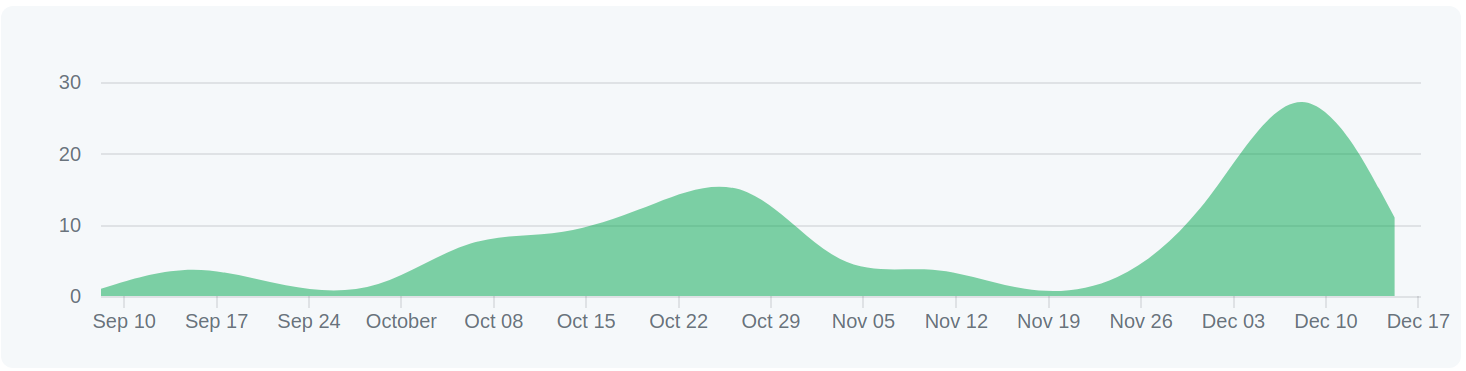
\includegraphics[scale=0.37]{github-timeline}

  \section {Team Roles and Responsibilities}
    The following table summarizes the major responsibilities taken up by each team member, with a number of components overlapping among team members.
    \begin{center}
      {\renewcommand{\arraystretch}{1.5}
      \begin{tabular}{|p{5cm}|p{10cm}|}
      \hline
      \textbf{Team Member} & \textbf{Responsibilities} \\
      \hline
      Aditya Narayanamoorthy (Language Guru) & Scanner, Parser, Ast, Semant, Sast, Codegen \\
      \hline
      Gergana Alteva (Project Manager) & Scanner, Parser, Ast, Semant, Sast, Codegen \\
      \hline
      Erik Dyer (System Architect) & VM, Docker, Graphics Library researching (SDL2), testing \\
      \hline
      Kunal Baweja (Tester) & predefined library, SDL2, SDL2\_gfx, Automated and Manual Test suite, Travis CI \\
      \hline
      \end{tabular}
    \end{center}

  \section{Software Development Environment}
    The following software development tools, libraries and dependencies were used for developing SOL compiler by the team.
    \begin{enumerate}
      \itemsep 0em
      \item Ubuntu \texttt{15.04} VM setup with ocaml compiler, opam, llvm toolchain, and ocaml Llvm module for llvm bindings.
      \item Ocaml version: \texttt{4.02.3}
      \item LLVM dev library: \texttt{3.8}
      \item opam Llvm package (Ocaml Llvm bindings)
      \item Sublime text with \texttt{merlin(ocaml)} and \texttt{cppcheck(C99)} linters
      \item Version Control: \texttt{Github}
      \item Travis CI: Automated testing on \texttt{Ubuntu 16.04} environment (same dependency configurations)
    \end{enumerate}

  \section {Project Logs}
  Please see appendix \ref{git:log} for project logs in reverse chronological order of timeline.

\chapter{Architectural Design}
  We describe the compilation structure for a SOL program through SOL compiler in this chapter. This can be broken down into 3 phases:
  \begin{enumerate}
    \itemsep 0em

    \item Compile SOL program to LLVM IR bytecode representation
    \item Compile generated IR to architecture specific assembly code using LLVM compiler
    \item Compile and link against predefined static library to produce executable
  \end{enumerate}

  \begin{figure}[ht]
    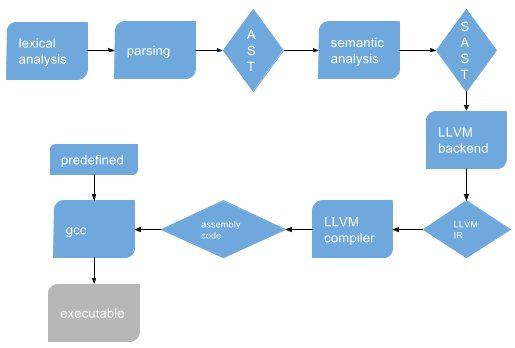
\includegraphics[scale=1]{compile-architecture.png}
    \caption{SOL Compiler Block Diagram}
  \end{figure}

  \section{Interfaces between SOL Compiler components}
    \subsection{Scanner}
      The scanner takes as input a \texttt{SOL(.sol) source program} and generates tokens for \textit{identifiers, keywords, operators, values, functions and shapes}, as specified by the lexical conventions for SOL in  Language Reference Manual (see chapter \ref{lrm}). It rejects a source program if it observes an invalid token, against the rules specified in \texttt{scanner.mll}

    \subsection{Parser}
      The parser accepts the tokenized output from scanner and generates an abstract syntax tree (AST) based on SOL syntax. It rejects the source program if a syntactic error is seen due to which a valid AST can not be generated.

    \subsection{Semantic Checker}
      The AST output from parser is passed to semantic checker to ensure semantic correctness of each program statement, including static type checking. Eg: An \texttt{int} variable can not be assigned a floating point value, per SOL specification. Such an assignment in SOL program will be semantically incorrect and rejected at the semantic checking phase.\\
      The semantic checking phase associates semantic information to the AST nodes and produces a SAST, if the program passes the semantic check.

    \subsection{Code Generation}
    The code generator accepts the SAST generated after semantic checking and generates the LLVM IR code using the OCaml Llvm bindings. The SOL \textit{primitives, arrays, shapes, functions, member functions} are all mapped to corresponding LLVM primitives, arrays, structs and function definitions representations.\\
    Once the LLVM IR code is generated successfully, the SOL compiler task is over. After this we use the LLVM compiler (\texttt{llc}) to convert the IR code to architecture specific assembly code. This is further compiled into an executable and statically linked against a predefined library, that interfaces with \texttt{SDL2} and \texttt{SDL2\_gfx}. 

    The compiler components were implemented by team members as listed below:
    \begin{center}
      {\renewcommand{\arraystretch}{1.5}
      \begin{tabular}{|p{5cm}|p{5cm}|p{5cm}|}
        \hline
        \textbf{Component} & \textbf{Source file} & \textbf{Team members} \\
        \hline
        Lexical Analysis & scanner.mll & Aditya, Gergana\\
        \hline
        Parsing & parser.mly & Aditya, Gergana\\
        \hline
        Abstract Syntax Tree & ast.ml & Aditya, Gergana\\
        \hline
        Semantic Analysis & semant.ml & Aditya, Gergana\\
        \hline
        SAST & sast.ml & Aditya, Gergana\\
        \hline
        LLVM backend & codegen.ml & Aditya, Gergana\\
        \hline
        Predefined graphic library & predefined.c & Kunal\\
        \hline
      \end{tabular}
    \end{center}

\chapter{Test Plan}
The SOL compiler was developed through a test driven development approach. 

  \section{Sample Programs}
  This section shows 3 sample programs written in SOL and corresponding LLVM IR code represtation generated for the source programs.
    \subsection{Recursive function}
    The following program shows a SOL program to print sum of natural numbers from 1 to \texttt{n}, where \texttt{n} is input to the program.

    \subsubsection{series.sol}
    \lstinputlisting[style=sol, aboveskip=2pt]{series.sol}

    \subsubsection{series.ll}
    \lstinputlisting[style=sol, aboveskip=2pt]{series.ll}

    \subsection{Composite Shape Drawing}
    The following program demonstrates construction of complex shapes in SOL. It defines two generic shapes, \texttt{Polygon} and \texttt{Spokes}. Further it uses \texttt{Polygon} to define a \texttt{Square} and defines a \texttt{FerrisWheel} shape using member variables of \texttt{Polygon}, \texttt{Square} and \texttt{Spokes} shapes. In the \texttt{draw} function of \texttt{FerrisWheel} we define the logic to draw the object at each frame, gradually speeding up the rotation speed, staying constant at that speed and then slowing down to a halt.

    \subsubsection{ferris-wheel.sol}
    \lstinputlisting[style=sol, aboveskip=2pt]{ferris-wheel.sol}

    \subsubsection{ferris-wheel.ll}
    \lstinputlisting[style=sol, aboveskip=2pt]{ferris-wheel.ll}

    \subsection{Animating Shapes}
    In this sample program, the introduction scene from \texit{James Bond} movie franchise is recreated, again defining two basic shapes, \texttt{Polygon} and \texttt{Line} and using these shapes to create circles for the screen and additionally define a \textit{Person} shape. For each of the objects created, a render block is defined which dictates the translation of individual objects.

    \subsubsection{james-bond.sol}
    \lstinputlisting[style=sol, aboveskip=2pt]{james-bond.sol}

    \subsubsection{james-bond.ll}
    \lstinputlisting[style=sol, aboveskip=2pt]{james-bond.ll}    

  \section{Test Suite}
    The test suite is divided into two major categories:
    \begin{itemize}
      \itemsep 0em
      \item Automated Tests - run on Travis CI
      \item Manual Tests - visually inspected for display correctness
    \end{itemize}

    \textbf{NOTE:} Please refer to \underline{Appendix \ref{test-suite}} for complete code listing of test cases.\\

    Test cases were written based on the syntactic and semantic specifications of language mentioned in SOL Language Reference Manual (chapter \ref{lrm}). This acted as a reference point for the team and allowed us to stay as close to the LRM specifications as practically possible throughout the compiler development process.\\

    The initial tests for each feature were written as \textit{functional tests} which would ensure the correct working of the feature once it was implemented and integrated into the compiler. Once the feature was integrated into compiler, it was put through the complete list of tests, automated, to ensure that the new changes did not adversely affect any of the previously implemented features and to verify that as part of the language, each individual feature works in a certain expected manner without any conflicts.\\

    We tested the following major components of our language, crucial for SOL:
    \begin{itemize}
      \itemsep 0em
      \item \textit{primitives} - The tests cover declaration and assignments of primitive variables extensively, through specific test cases for assignment, operations, declarations, scoping rules and static type checking.

      \item \textit{Arrays} - Fixed size arrays of primitives are supported by SOL and hence we extensively tested for array declaration, assigning and accessing individual elements. SOL does not provide bounds checking, much like C and hence it is programmer's responsibility to ensure that.

      \item \textit{Shapes} - Defining shapes for drawing and animation on screen is the basic feature of object-oriented paradigm supported by SOL. We tested defining, instantiating and animating shapes through multiple automated and manual test cases, for visual correctness of rendered drawings. This includes defining and creating complex shapes using simpler shape definitions.

      \item \textit{Operations} - SOL allows basic arithmetic and logical operations on integers and floating point numbers and these have been tested with respect to order of precedence and associativity rules in an expression, alongside correctness of result output by each individual operation.

      \item \textit{Functions} - SOL supports declaring functions, both standalone as well as member functions of a shape. These have been tested by checking for return types, values, recursion, expected number of arguments and argument types, syntactic correctness and expected failures in case of incorrect source programs.

      \item \textit{Type Conversion} - SOL allows converting, \texttt{int}, \texttt{float} and \texttt{char} values to \texttt{string} through appropriate functions mentioned in the Language Reference Manual and tested via \texttt{consolePrint} and \texttt{print} function calls.

      \item \textit{Drawing Function} - Three basic drawing functions are provided as built-ins by SOL for rendering text and shapes on screen. These have been tested through manual testcases, wherein a visual inspection of displayed content is required to ensure correctness.

      \item \textit{Output Function} - Apart from the drawing functions mentioned above, the only output function provided is \texttt{consolePrint}} which outputs the \texttt{string} argument to standard output and tested by comparing the outputs against expected outputs of corresponding test programs.

      \item \textit{Animation Function} - The \textit{translate} and \textit{rotate} functions are the basic components that allow a SOL programmer to animate objects and these have been tested for intended behaviour rigorously to account for intended and possible unintended side effects of the program written.
  \end{itemize}

  \section{Test Automation}
    We used \textit{Travis CI} in conjunction with the \texttt{testall.sh} script (see \ref{test-suite}) for automatically running all test cases and checking outputs against the expected output from the compiled program or failure during compilation or runtime of program. Setting up Travis CI allowed us to run the complete regression test suite in a standardized development environment, for every code push to the github repository, without manual intervention and be notified in case of test failures.

  \section{Manual Testing}
    Testing shape display and animation correctness was not possible within \texit{Travis CI} environment as it does not support a display console for  testing. These test cases were written separately, in test files following tnaming pattern \texttt{mnl-*}, compiled and run using the same test script, although these required manual intervention for correctness of displayed graphics. Please see Appendix \ref{mnl-test} for manual test cases.

  \section{Testing Responsibilities}
  \begin{center}
    {\renewcommand{\arraystretch}{1.5}
    \begin{tabular}{|p{5cm}|p{8cm}|}
      \hline
      \textbf{Team member} & \textbf{Responsibilties}\\
      \hline
      Kunal Baweja (Tester) & Test Plan, Travis CI/Automation, Test environment setup, Writing regression \& unit tests\\
      \hline
      Erik Dyer (System Architect) & Writing regression \& unit tests\\
      \hline
    \end{tabular}
  \end{center}

\chapter{Lessons Learned}
  
  \section{Aditya Narayanmoorthy}

  \section{Erik Dyer}
    This semester I learned how important organization and communication is. I think one thing that was really good about our team is that we were very good about sticking to meeting frequently from the beginning. Having this organization from the beginning allowed us to avoid the \"who\'s free to meet when?\" dance and therefore build up an early momentum that was sustained throughout the semester.\\

    I think that one piece of advice I'd give to future groups is to think about what kind of language you could build from before you take the class. Our group took several meetings before we decided what kind of language we wanted to have, and that\'s before we even got to the language details. Coming in with a language idea will definitely be helpful and save time.

  \section{Gegana Alteva}
    Building a compiler in a team has provided me with many lessons throughout the semester. My development experience is limited and while I had an understanding of what needed to be done, I was not sure how it should be done. I learned the importance of implementing our language vertically and how to prioritize components. My advice for future teams would be to prioritize what needs to be implemented by understanding what is absolutely needed for your language to work. There are many language design aspects that seem necessary, but in reality are just \"nice-to-have\"s. Had I done a better job of prioritizing and classifying what is and is not a \"nice-to-have\", we would have perhaps spent more time coding what was actually needed.

  \section{Kunal Baweja}
% Appendix code listings
\begin{appendices}

\chapter{SOL Compiler}

Code listing for compiler code. Author names are mentioned as first comment line of each code listing.

    \section{scanner.mll}
    \lstinputlisting[style=caml]{../scanner.mll}

    \section{parser.mly}
    \lstinputlisting[style=caml]{../parser.mly}

    \section{ast.ml}
    \lstinputlisting[style=caml]{../ast.ml}

    \section{semant.ml}
    \lstinputlisting[style=caml]{../semant.ml}

    \section{sast.ml}
    \lstinputlisting[style=caml]{../sast.ml}

    \section{codegen.ml}
    \lstinputlisting[style=caml]{../codegen.ml}

    \section{sol.ml}
    \lstinputlisting[style=caml]{../codegen.ml}

    \section{predefined.h}
    \lstinputlisting[style=caml]{../predefined.h}

    \section{predefined.c}
    \lstinputlisting[style=caml]{../predefined.c}

    \section{Makefile}
    \lstinputlisting[style=make]{../Makefile}


\chapter{Environment Setup}

The following scripts can be used for installing dependencies and setting up environment.

    \section{install-llvm.sh}
    \lstinputlisting[style=bash]{../install-llvm.sh}

    \section{install-sdl-gfx.sh}
    \lstinputlisting[style=bash]{../install-sdl-gfx.sh}

\chapter{Automated testing}\label{test-suite}

The first two scripts are used for automated testing on Travis CI. For individual test cases, the author names are mentioned as first line of each test case.

    \section{.travis.yml}
    \lstinputlisting[style=bash]{../.travis.yml}

    \section{testall.sh}
    \lstinputlisting[style=bash]{../testall.sh}

    %% include latest set of automated test files
    %% use g.py scrip to generate the test-case.tex
    %% recompile the latex document
    \section{fail-array-assign.sol}
\lstinputlisting[style=sol,aboveskip=-4pt]{../tests/fail-array-assign.sol}

\section{test-array-of-shape.sol}
\lstinputlisting[style=sol,aboveskip=-4pt]{../tests/test-array-of-shape.sol}

\section{test-char-to-string.sol}
\lstinputlisting[style=sol,aboveskip=-4pt]{../tests/test-char-to-string.sol}

\section{fail-div-semantic.sol}
\lstinputlisting[style=sol,aboveskip=-4pt]{../tests/fail-div-semantic.sol}

\section{test-add.sol}
\lstinputlisting[style=sol,aboveskip=-4pt]{../tests/test-add.sol}

\section{test-precedence.sol}
\lstinputlisting[style=sol,aboveskip=-4pt]{../tests/test-precedence.sol}

\section{test-if.sol}
\lstinputlisting[style=sol,aboveskip=-4pt]{../tests/test-if.sol}

\section{fail-prod-semantic.sol}
\lstinputlisting[style=sol,aboveskip=-4pt]{../tests/fail-prod-semantic.sol}

\section{test-empty-function.sol}
\lstinputlisting[style=sol,aboveskip=-4pt]{../tests/test-empty-function.sol}

\section{test-shape-member-shape.sol}
\lstinputlisting[style=sol,aboveskip=-4pt]{../tests/test-shape-member-shape.sol}

\section{fail-array-access-pos.sol}
\lstinputlisting[style=sol,aboveskip=-4pt]{../tests/fail-array-access-pos.sol}

\section{fail-parameter-floatint.sol}
\lstinputlisting[style=sol,aboveskip=-4pt]{../tests/fail-parameter-floatint.sol}

\section{fail-recursion.sol}
\lstinputlisting[style=sol,aboveskip=-4pt]{../tests/fail-recursion.sol}

\section{test-while.sol}
\lstinputlisting[style=sol,aboveskip=-4pt]{../tests/test-while.sol}

\section{fail-return-void-int.sol}
\lstinputlisting[style=sol,aboveskip=-4pt]{../tests/fail-return-void-int.sol}

\section{test-function-shape-formal.sol}
\lstinputlisting[style=sol,aboveskip=-4pt]{../tests/test-function-shape-formal.sol}

\section{test-product.sol}
\lstinputlisting[style=sol,aboveskip=-4pt]{../tests/test-product.sol}

\section{fail-array-access-neg.sol}
\lstinputlisting[style=sol,aboveskip=-4pt]{../tests/fail-array-access-neg.sol}

\section{test-logical.sol}
\lstinputlisting[style=sol,aboveskip=-4pt]{../tests/test-logical.sol}

\section{test-escape-chars.sol}
\lstinputlisting[style=sol,aboveskip=-4pt]{../tests/test-escape-chars.sol}

\section{fail-return-int-string.sol}
\lstinputlisting[style=sol,aboveskip=-4pt]{../tests/fail-return-int-string.sol}

\section{test-array-pass-ref.sol}
\lstinputlisting[style=sol,aboveskip=-4pt]{../tests/test-array-pass-ref.sol}

\section{test-int-to-string.sol}
\lstinputlisting[style=sol,aboveskip=-4pt]{../tests/test-int-to-string.sol}

\section{test-shape-function.sol}
\lstinputlisting[style=sol,aboveskip=-4pt]{../tests/test-shape-function.sol}

\section{test-float-to-string.sol}
\lstinputlisting[style=sol,aboveskip=-4pt]{../tests/test-float-to-string.sol}

\section{test-framerate.sol}
\lstinputlisting[style=sol,aboveskip=-4pt]{../tests/test-framerate.sol}

\section{fail-if.sol}
\lstinputlisting[style=sol,aboveskip=-4pt]{../tests/fail-if.sol}

\section{test-shape-array.sol}
\lstinputlisting[style=sol,aboveskip=-4pt]{../tests/test-shape-array.sol}

\section{test-trigono-func.sol}
\lstinputlisting[style=sol,aboveskip=-4pt]{../tests/test-trigono-func.sol}

\section{fail-func-arg.sol}
\lstinputlisting[style=sol,aboveskip=-4pt]{../tests/fail-func-arg.sol}

\section{fail-add-semantic.sol}
\lstinputlisting[style=sol,aboveskip=-4pt]{../tests/fail-add-semantic.sol}

\section{test-hello.sol}
\lstinputlisting[style=sol,aboveskip=-4pt]{../tests/test-hello.sol}

\section{fail-assign-stringint.sol}
\lstinputlisting[style=sol,aboveskip=-4pt]{../tests/fail-assign-stringint.sol}

\section{test-assign-variable.sol}
\lstinputlisting[style=sol,aboveskip=-4pt]{../tests/test-assign-variable.sol}

\section{test-set-array.sol}
\lstinputlisting[style=sol,aboveskip=-4pt]{../tests/test-set-array.sol}

\section{test-array-assign.sol}
\lstinputlisting[style=sol,aboveskip=-4pt]{../tests/test-array-assign.sol}

\section{test-comparison.sol}
\lstinputlisting[style=sol,aboveskip=-4pt]{../tests/test-comparison.sol}

\section{fail-add-intstring.sol}
\lstinputlisting[style=sol,aboveskip=-4pt]{../tests/fail-add-intstring.sol}

\section{test-recursion.sol}
\lstinputlisting[style=sol,aboveskip=-4pt]{../tests/test-recursion.sol}

\section{test-division.sol}
\lstinputlisting[style=sol,aboveskip=-4pt]{../tests/test-division.sol}

\section{test-associativity.sol}
\lstinputlisting[style=sol,aboveskip=-4pt]{../tests/test-associativity.sol}

\section{test-math-round.sol}
\lstinputlisting[style=sol,aboveskip=-4pt]{../tests/test-math-round.sol}

\section{test-shape-define.sol}
\lstinputlisting[style=sol,aboveskip=-4pt]{../tests/test-shape-define.sol}

\section{test-array-access.sol}
\lstinputlisting[style=sol,aboveskip=-4pt]{../tests/test-array-access.sol}

\section{test-float-to-int.sol}
\lstinputlisting[style=sol,aboveskip=-4pt]{../tests/test-float-to-int.sol}

\section{test-int-to-float.sol}
\lstinputlisting[style=sol,aboveskip=-4pt]{../tests/test-int-to-float.sol}



\chapter{Manual Testing}\label{mnl-test}

  \section{mnl-composite-square.sol}
\lstinputlisting[style=sol,aboveskip=-4pt]{../tests/manual/mnl-composite-square.sol}

\section{mnl-drawpoint.sol}
\lstinputlisting[style=sol,aboveskip=-4pt]{../tests/manual/mnl-drawpoint.sol}

\section{mnl-translate-triangle.sol}
\lstinputlisting[style=sol,aboveskip=-4pt]{../tests/manual/mnl-translate-triangle.sol}

\section{mnl-polygon-collision.sol}
\lstinputlisting[style=sol,aboveskip=-4pt]{../tests/manual/mnl-polygon-collision.sol}

\section{mnl-polygon.sol}
\lstinputlisting[style=sol,aboveskip=-4pt]{../tests/manual/mnl-polygon.sol}

\section{mnl-planet.sol}
\lstinputlisting[style=sol,aboveskip=-4pt]{../tests/manual/mnl-planet.sol}

\section{mnl-collision.sol}
\lstinputlisting[style=sol,aboveskip=-4pt]{../tests/manual/mnl-collision.sol}

\section{mnl-disco-bar.sol}
\lstinputlisting[style=sol,aboveskip=-4pt]{../tests/manual/mnl-disco-bar.sol}

\section{mnl-hello.sol}
\lstinputlisting[style=sol,aboveskip=-4pt]{../tests/manual/mnl-hello.sol}

\section{mnl-line.sol}
\lstinputlisting[style=sol,aboveskip=-4pt]{../tests/manual/mnl-line.sol}

\section{mnl-thick-line.sol}
\lstinputlisting[style=sol,aboveskip=-4pt]{../tests/manual/mnl-thick-line.sol}

\section{mnl-ferris-move.sol}
\lstinputlisting[style=sol,aboveskip=-4pt]{../tests/manual/mnl-ferris-move.sol}

\section{mnl-triangle.sol}
\lstinputlisting[style=sol,aboveskip=-4pt]{../tests/manual/mnl-triangle.sol}

\section{mnl-laser-collision.sol}
\lstinputlisting[style=sol,aboveskip=-4pt]{../tests/manual/mnl-laser-collision.sol}

\section{mnl-james-bond.sol}
\lstinputlisting[style=sol,aboveskip=-4pt]{../tests/manual/mnl-james-bond.sol}



\chapter{Commit Logs} \label{git:log}
  \lstinputlisting[style=make, stringstyle=\color{black}]{commit.log}

\end{appendices}

\end{document}
